\documentclass[../Main/Knit.tex]{subfiles}

\section{Introduction}
One current limitation of whole transcriptome sequencing is the low coverage/sequencing depth achieved per gene due to the distribution of reads across the whole transcriptome. Consequently, while whole transcriptome sequencing allows identification of novel genes (genes not previously annotated to the genome) and novel isoforms, it may not detect isoforms particularly those of low expression resulting in many false negatives. This can be circumvented by the use of target capture, which enriches a selective panel of genes that are then only sequenced. Multiple samples can further be pooled and sequenced together by barcoding samples at cDNA synthesis, which simplifies laboratory workflow and minimises associated sequencing costs.

%[Other methods of Targeted Sequencing i.e. CRISPR]

%Advantages of targeted transcriptomics vs whole transcriptomics; resources in Targeted Transcriptomics paper; Literature Review 
%List of relevance of AD genes


\section{Methods}
The extracted RNA from mouse rTg4510 samples were prepared for targeted transcriptome sequencing on the PacBio's Sequel (n = 24, Table \ref{tab:mouse_samples_sequenced}), a subset of which were also sequenced on the Oxford Nanopore's MinION (n = 18, Table \ref{tab:mouse_samples_sequenced}). Three biological replicates were selected at each age (2, 4, 6 and 8 months) across wildtype and transgenic mice, multiplexed using barcodes (listed in Table \ref{tab:barcode_primers}) and ran on the Sequel as three batches. Iso-Seq library preparation and SMRT sequencing is described in Chapter X. 

\begin{landscape}
\begin{table}[]
		\resizebox{1.5\textwidth}{!}{%
	\begin{tabular}{@{}cccccccccc@{}}
		\toprule
		\multicolumn{6}{c}{\multirow{2}{*}{\begin{tabular}[c]{@{}c@{}}Sample   \\ demographics\end{tabular}}} &
		\multicolumn{4}{c}{Sequencing Platform} \\ \cmidrule(l){7-10} 
		\multicolumn{6}{c}{}                      & \multicolumn{2}{c}{PacBio Iso-Seq} & \multicolumn{2}{c}{Oxford Nanopore} \\ \midrule
		Sample &
		Phenotype &
		Age (Months) &
		RIN &
		\begin{tabular}[c]{@{}c@{}}Concentration\\ (ng/ul)\end{tabular} &
		\begin{tabular}[c]{@{}c@{}}Batch \\ (Barcodes)\end{tabular} &
		\begin{tabular}[c]{@{}c@{}}Whole \\ Transcriptome\end{tabular} &
		\begin{tabular}[c]{@{}c@{}}Targeted\\  Transcriptome\end{tabular} &
		\begin{tabular}[c]{@{}c@{}}Whole \\ Transcriptome\end{tabular} &
		\begin{tabular}[c]{@{}c@{}}Targeted \\ Transcriptome\end{tabular} \\ \midrule
		K19 & WT & 4 & 8.8 & 236  & 1 (PB\_BC\_1) &                 & X               &                  &                  \\
		K23 & WT & 8 & 9.1 & 143  & 1 (PB\_BC\_2) & X               & X               &                  &                  \\
		K21 & WT & 6 & 9   & 138  & 1 (PB\_BC\_3) &                 & X               &                  &                  \\
		K18 & TG & 2 & 8.8 & 136  & 1 (PB\_BC\_4) & X               & X               & X                &                  \\
		K20 & TG & 4 & 9.1 & 80.4 & 1 (PB\_BC\_5) &                 & X               &                  &                  \\
		K17 & WT & 2 & 9.2 & 77.1 & 1 (PB\_BC\_6) & X               & X               &                  &                  \\
		S19 & WT & 4 & 9.1 & 84.9 & 2 (PB\_BC\_1) &                 & X               &                  & X                \\
		K24 & TG & 8 & 9.2 & 65.4 & 2 (PB\_BC\_2) & X               & X               &                  & X                \\
		L22 & TG & 8 & 8.7 & 68.6 & 2 (PB\_BC\_3) & X               & X               &                  & X                \\
		M21 & WT & 2 & 9.2 & 72.3 & 2 (PB\_BC\_4) & X               & X               & X                & X                \\
		O18 & TG & 2 & 8.9 & 115  & 2 (PB\_BC\_5) & X               & X               &                  & X                \\
		O23 & WT & 8 & 9   & 91.8 & 2 (PB\_BC\_6) & X               & X               &                  & X                \\
		O22 & TG & 6 & 9.1 & 83.5 & 2 (PB\_BC\_7) &                 & X               &                  & X                \\
		P19 & WT & 6 & 8.9 & 92.2 & 2 (PB\_BC\_8) &                 & X               &                  & X                \\
		T20 & TG & 6 & 9   & 68.7 & 2 (PB\_BC\_9) &                 & X               &                  & X                \\
		Q20 & TG & 8 & 8.6 & 99.7 & 3 (PB\_BC\_1) & X               & X               &                  & X                \\
		Q21 & WT & 2 & 9.2 & 83.3 & 3 (PB\_BC\_2) & X               & X               &                  & X                \\
		S18 & TG & 2 & 8.9 & 115  & 3 (PB\_BC\_3) & X               & X               &                  & X                \\
		S23 & WT & 8 & 9.1 & 95.5 & 3 (PB\_BC\_4) & X               & X               &                  & X                \\
		Q18 & TG & 6 & 8.8 & 87.2 & 3 (PB\_BC\_5) &                 & X               &                  & X                \\
		Q17 & WT & 6 & 8.7 & 85.8 & 3 (PB\_BC\_6) &                 & X               &                  & X                \\
		L18 & TG & 4 & 8.8 & 145  & 3 (PB\_BC\_7) &                 & X               &                  & X                \\
		Q23 & WT & 4 & 9   & 70.8 & 3 (PB\_BC\_8) &                 & X               &                  & X                \\
		T18 & TG & 4 & 9   & 85   & 3 (PB\_BC\_9) &                 & X               &                  & X                \\ \bottomrule
	\end{tabular}%
}
\captionsetup{width=1.5\textwidth}
\caption[Mouse rTg4510 samples sequenced using whole and targeted transcriptome approach with PacBio Iso-Seq and ONT nanopore sequencing]%
{Mouse rTg4510 samples sequenced using whole and targeted transcriptome approach with PacBio Iso-Seq and ONT nanopore sequencing}
\label{tab:mouse_samples_sequenced}
\end{table}
\end{landscape}
\begin{table}[ht]
	\begin{tabular}{@{}cccccc@{}}
		\toprule
		Target &
		\begin{tabular}[c]{@{}c@{}}Number \\ of \\ Probes\end{tabular} &
		\begin{tabular}[c]{@{}c@{}}Genome \\ Co-ordinates\end{tabular} &
		Strand &
		\begin{tabular}[c]{@{}c@{}}Full\\  Region\\  (bp)\end{tabular} &
		\begin{tabular}[c]{@{}c@{}}Exons inc UTR \\ (bp)\end{tabular} \\ \midrule
		ABCA1  & 56         & chr  4 : 53030670 -   53160014    & - & 129,107 & 10,260 \\
		ABCA7  & 47         & chr  10 : 79997615 -   80015572   & + & 17,958  & 6,594  \\
		ANK1   & 52         & chr  8 : 22974836 -   23150497    & + & 175,662 & 9,018  \\
		APOE   & 5          & chr  7 : 19696125 -   19699285    & - & 2,923   & 1,251  \\
		APP    & 20         & chr  16 : 84954317 -   85173826   & - & 219,272 & 3,357  \\
		BIN1   & 20         & chr  18 : 32377217 -   32435740   & + & 58,524  & 2,455  \\
		CD33   & 9          & chr  7 : 43528610 -   43533290    & - & 5,716   & 2,571  \\
		CLU    & 9          & chr  14 : 65968483 -   65981545   & + & 13,063  & 1,808  \\
		FUS    & 16         & chr  7 : 127967479 -   127982032  & + & 14,554  & 1,845  \\
		FYN    & 18         & chr  10 : 39369799 -   39565381   & + & 195,583 & 3,692  \\
		MAPT   & 23         & chr  11 : 104231436 -   104332096 & + & 100,661 & 5,387  \\
		PICALM & 24         & chr  7 : 90130232 -   90209447    & + & 79,216  & 4,174  \\
		PTK2B  & 32         & chr  14 : 66153138 -   66281171   & - & 127,796 & 4,034  \\
		RHBDF2 & 21         & chr  11 : 116598082 -   116627138 & - & 28,855  & 3,934  \\
		SNCA   & 7          & chr  6 : 60731454 -   60829974    & - & 98,283  & 1,463  \\
		SORL1  & 48         & chr  9 : 41968370 -   42124408    & - & 155,801 & 6,938  \\
		TARDBP & 15         & chr  4 : 148612263 -   148627115  & - & 14,615  & 7,454  \\
		TREM2  & 5          & chr  17 : 48346401 -   48352276   & + & 5,876   & 1,146  \\
		TRPA1  & 28         & chr  1 : 14872529 -   14918981    & - & 46,215  & 4,263  \\
		VGF    & 9          & chr  5 : 137030295 -   137033351  & + & 3,057   & 2,553  \\
		& Total: 464 &                                   &   &         &        \\ \bottomrule
	\end{tabular}
\end{table}

\section{Results}
\subsection{Run performance and sequencing metrics}
Following library preparation and SMRT sequencing, a total of XXGb (s.d = XXGb) were obtained (Table \ref{tab:targeted_mouse_run_output}). Of note, 6 samples were first trialled and multiplexed in Batch 1 to determine the yield output and coverage depth - PacBio recommends starting with 4 - 8 samples for multiplexing. Having noticed that an average yield output (24Gb) with a high off-target sequencing, implicating saturation of target genes with 6 samples, the number was increased to 9 samples in Batch 2 and Batch 3. Despite more samples, the sequencing run for Batch 2 and 3, performed by Exeter's Seqeuncing Service, had a poor loading rate (38.1\% P1 of Batch 3 vs 71\% of Batch 1) and low subsequent yield. The samples were also potentially degraded after having been stored in -20\textdegree C for over 6 months due to Covid-19 lockdown. 

\begin{landscape}
	\begin{table}[]
		\resizebox{1.5\textwidth}{!}{%
			\begin{tabular}{@{}cccccccccccccccccccl@{}}
				\toprule
				\multirow{3}{*}{Sample} &
				\multirow{3}{*}{\begin{tabular}[c]{@{}c@{}}Total \\ Bases \\ (GB)\end{tabular}} &
				\multirow{3}{*}{\begin{tabular}[c]{@{}c@{}}Polymerase\\ Reads\end{tabular}} &
				\multicolumn{6}{c}{Read   Length} &
				\multicolumn{3}{c}{Productivity} &
				\multicolumn{4}{c}{Control} &
				\multirow{3}{*}{\begin{tabular}[c]{@{}c@{}}Local \\ Base \\ Rate\end{tabular}} &
				\multicolumn{2}{c}{Template} &
				\multicolumn{1}{c}{\multirow{3}{*}{Notes}} \\ \cmidrule(lr){4-16} \cmidrule(lr){18-19}
				&
				&
				&
				\multicolumn{2}{c}{Polymerase} &
				\multicolumn{2}{c}{Subread} &
				\multicolumn{2}{c}{Insert} &
				\multirow{2}{*}{P0} &
				\multirow{2}{*}{P1} &
				\multirow{2}{*}{P2} &
				\multirow{2}{*}{\begin{tabular}[c]{@{}c@{}}Total   \\ Reads\end{tabular}} &
				\multirow{2}{*}{\begin{tabular}[c]{@{}c@{}}Read \\ Length\\  Mean\end{tabular}} &
				\multicolumn{2}{c}{Concordance} &
				&
				\multirow{2}{*}{\begin{tabular}[c]{@{}c@{}}Adapter   \\ Dimer \\ (0-10bp)\end{tabular}} &
				\multirow{2}{*}{\begin{tabular}[c]{@{}c@{}}Short \\ Insert \\ (11-100bp)\end{tabular}} &
				\multicolumn{1}{c}{} \\ \cmidrule(lr){4-9} \cmidrule(lr){15-16}
				&
				&
				&
				Mean &
				N50 &
				Mean &
				N50 &
				Mean &
				N50 &
				&
				&
				&
				&
				&
				Mean &
				Mode &
				&
				&
				&
				\multicolumn{1}{c}{} \\ \midrule
				Batch 1 &
				24.2 &
				712250 &
				34016 &
				70473 &
				1402 &
				1852 &
				3024 &
				3808 &
				\begin{tabular}[c]{@{}c@{}}4.62\% \\ (46613)\end{tabular} &
				\begin{tabular}[c]{@{}c@{}}71.58\%\\  (722026)\end{tabular} &
				\begin{tabular}[c]{@{}c@{}}24.76\% \\ (249707)\end{tabular} &
				9,690 &
				31,505 &
				0.84 &
				0.87 &
				2.31 &
				0 &
				0 &
				Sequenced in November 2019 \\
				Batch 2 &
				&
				&
				&
				&
				&
				&
				&
				&
				&
				&
				&
				&
				&
				&
				&
				&
				&
				&
				\multirow{2}{*}{\begin{tabular}[c]{@{}l@{}}Sequenced in July 2020\\ Samples were kept at -20 for over 9months. \\ Sequel broke down mid-run.  \\ Sequencing was prepared by Exeter's Sequencing Services\\ \\ \end{tabular}} \\
				Batch 3 &
				19.3 &
				383292 &
				50472 &
				100255 &
				1557 &
				2017 &
				3158 &
				3898 &
				\begin{tabular}[c]{@{}c@{}}18.68\% \\ (189549)\end{tabular} &
				\begin{tabular}[c]{@{}c@{}}38.11\%\\  (386743)\end{tabular} &
				\begin{tabular}[c]{@{}c@{}}43.56\% \\ (442054)\end{tabular} &
				3,440 &
				52,533 &
				0.85 &
				0.87 &
				2.86 &
				0 &
				0 &
				\\ \bottomrule
			\end{tabular}%
		}
		\captionsetup{width=1.5\textwidth}
		\caption[Run Yield Output from Targeted Transcriptome Iso-Seq of Tg4510]%
		{Iso-Seq run yield for each batch of Tg4510 mouse samples sequenced using targeted transcriptome approach}
		\label{tab:targeted_mouse_run_output}
	\end{table}
\end{landscape}


The yield difference between the first and last two batches was evident in the number of CCS reads (total = 996K; Batch 1 = 469K, Batch 2 = 306K, Batch 3 = 2221K Figure \ref{fig:isoseq_targeted_run_output}a) and FLNC reads (total = 930K; Batch 1 = 399K, Batch 2 = 275K, Batch 3 = 256K, Figure \ref{fig:isoseq_targeted_run_output}a) generated, after applying the bioinformatics Iso-Seq pipeline (same as the whole transcriptome approach with the exception of removing barcodes rather than general primers). However, calculation of the on-target rate suggested that while Batch 2 and 3 had lower output yield, the coverage of target genes was significantly greater than Batch 1 due to the increased sample size (mean rate in Batch 1 = 34.5\%; mean rate in Batch 2 = 46.2\%; mean rate in Batch 3: 42.9\%, Figure \ref{fig:isoseq_targeted_rate}). The on-target rate is defined as the proportion of mapped transcripts with sequences overlapping at least one target probe. 
%Off-target 

In addition to batch variability, the number of full-length transcripts obtained per sample varied within each batch (Figure \ref{fig:isoseq_targeted_run_output}b). This variability was not associated with RIN (corr = 0.147, P = 0.492, Spearman's rank) and is unlikely to be due to library preparation, given that samples were pooled in equal molarity during target capture. However, there was no significant difference in the number of full-length transcripts between WT and TG across the batched runs (Wilcoxon rank sum test, W = 73, P = 0.977, Figure \ref{fig:isoseq_targeted_run_output}c). 



\begin{figure}[!htb]
	\begin{center}
		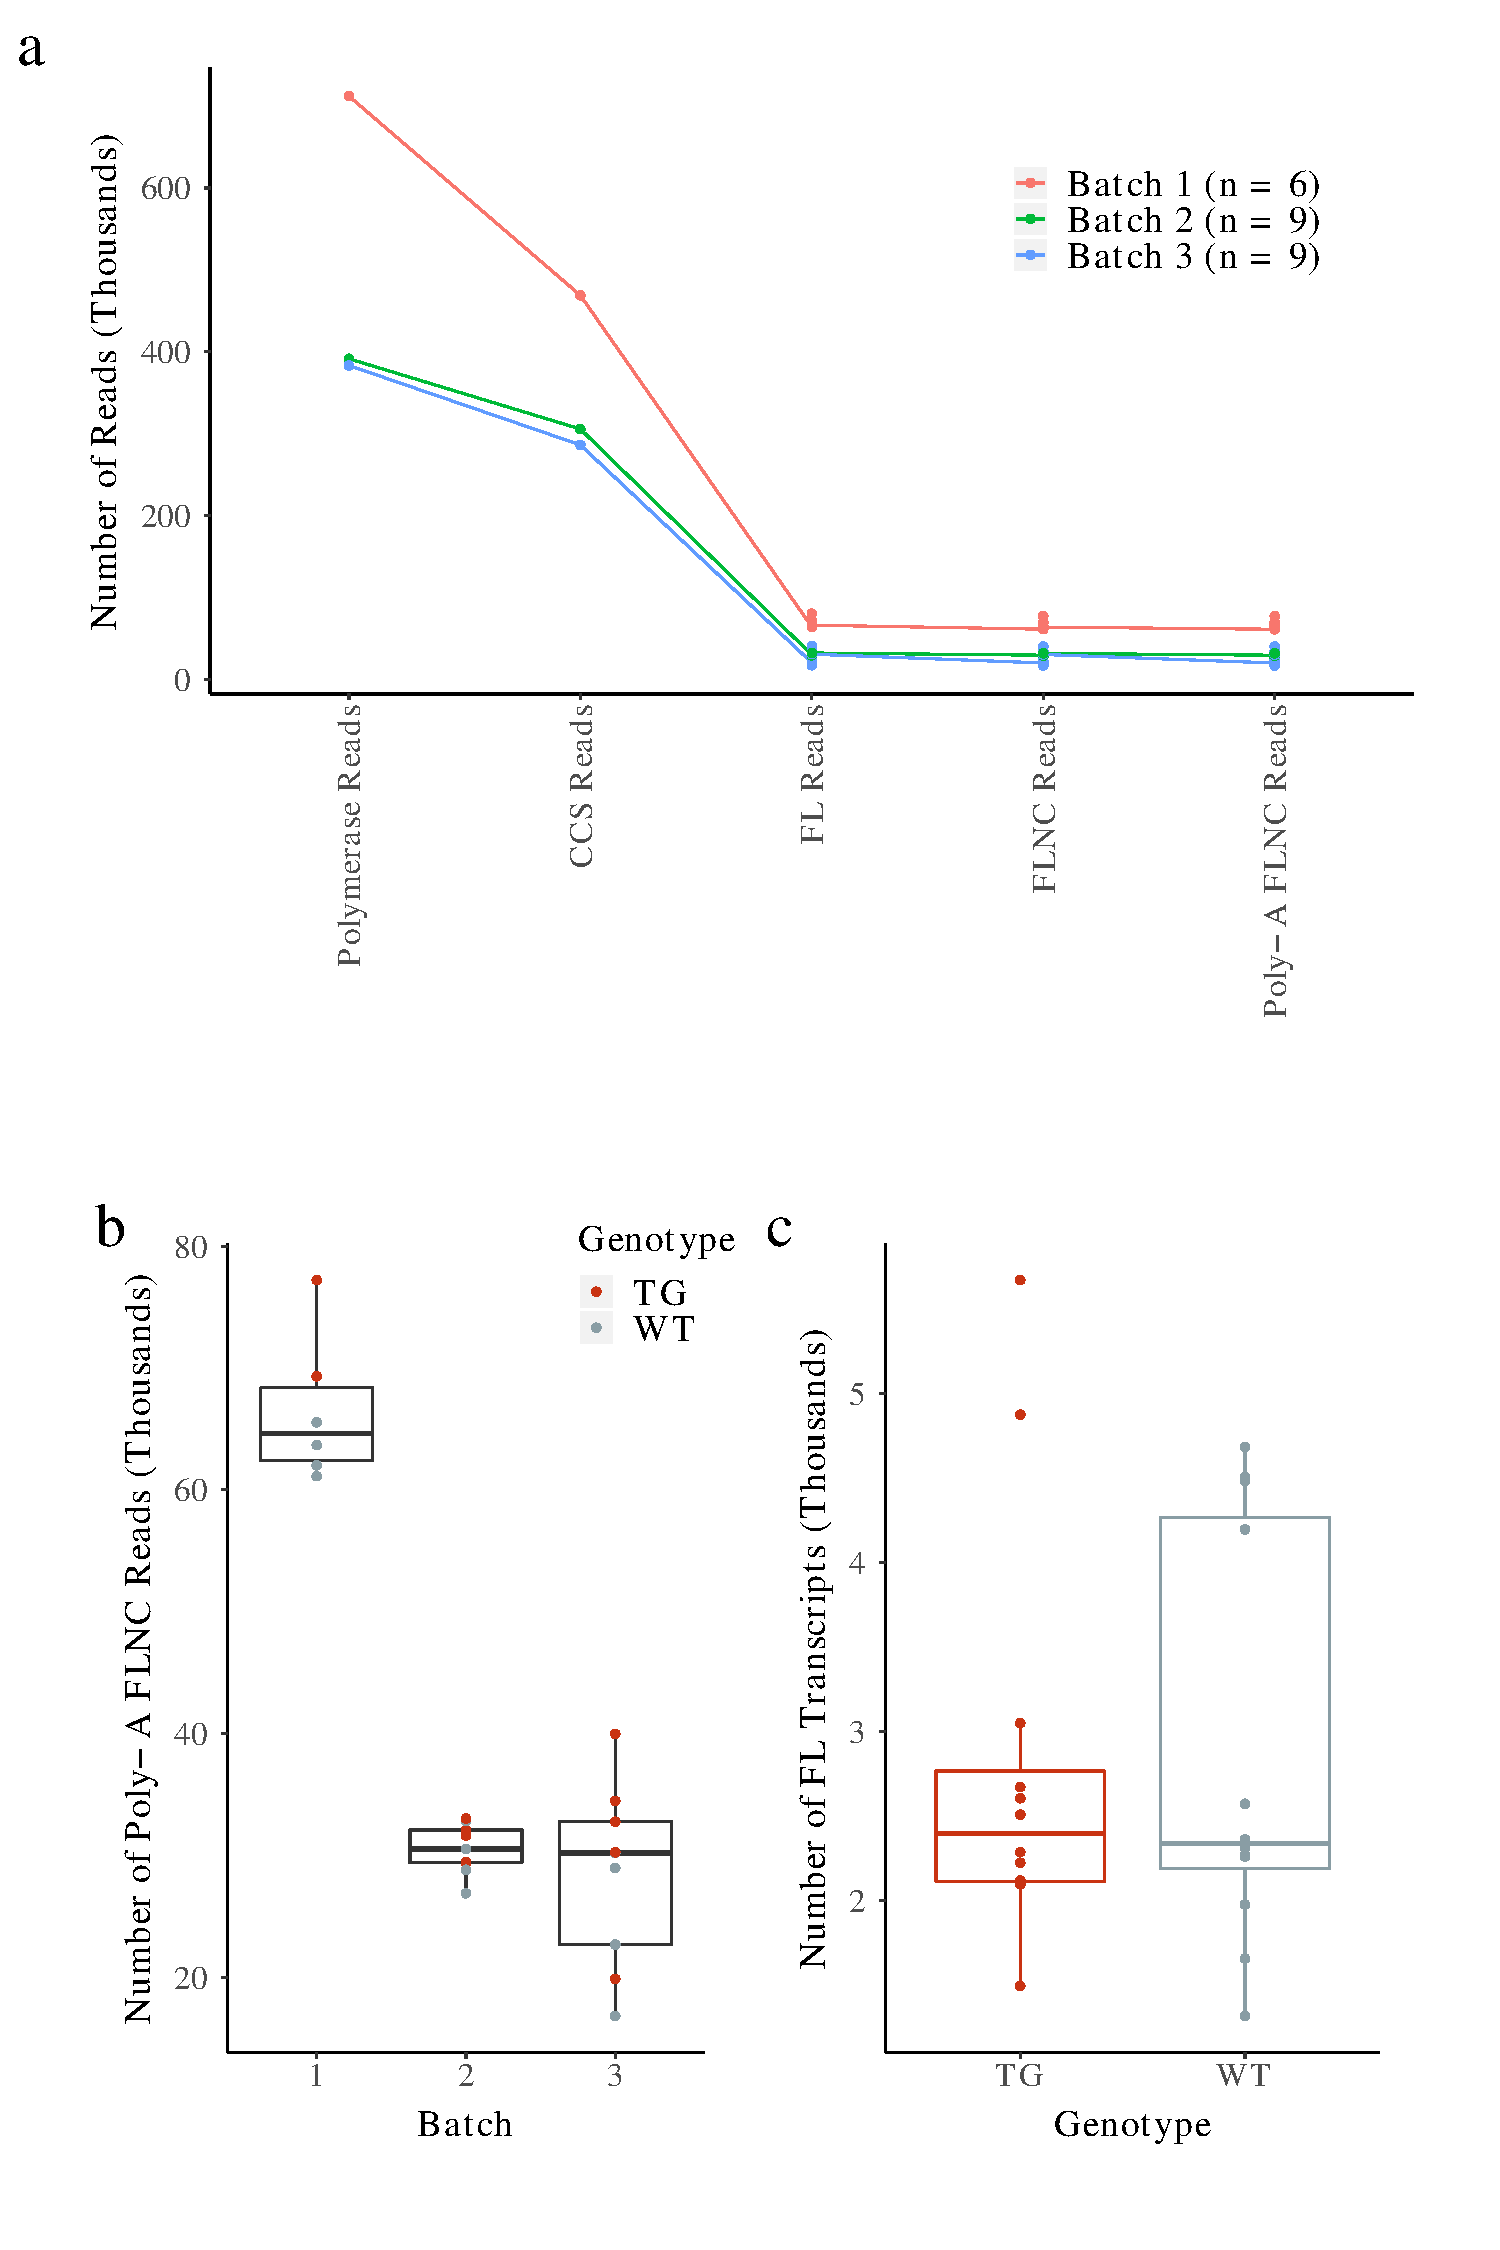
\includegraphics[page=1,trim={0 1cm 0 0},clip,scale = 0.55]{TargetedTranscriptome.pdf}
	\end{center}
	\captionsetup{width=0.95\textwidth}
	\caption[Targeted Transcriptome Iso-seq run performance]%
	{\textbf{Despite batch variability in targeted transcriptome sequencing, no difference in the number of full-length transcripts was observed between wildtype and transgenic mice}. \textbf{a)} Samples (n = 24) were multiplexed and sequenced in three runs (Batch 1, 2 and 3) with varied performance, as indicated by the number of polymerase reads through to poly-A FLNC reads. In the bioinformatics pipeline, the samples were demultiplexed and individually processed after generation of CCS reads from each run. \textbf{b)} Sample variability within each batch was observed from the number of poly-A FLNC reads generated. However, \textbf{c)} no statistical difference was observed in the overall number of full-length transcripts detected between wildtype and transgenic. Full-length transcripts were collapsed from poly-A FLNC reads in Iso-Seq Cluster. CCS - Circular Consensus Sequence, FLNC - Full-Length Non-Concatemer, FL - Full-Length, WT - Wildtype, TG - Transgenic}
	\label{fig:isoseq_targeted_run_output}
\end{figure}

\begin{figure}[!htb]
	\begin{center}
		\includegraphics[page=2,trim={0 25cm 0 0},clip,scale = 0.55]{TargetedTranscriptome.pdf}
	\end{center}
	\captionsetup{width=0.95\textwidth}
	\caption[On-Target rate in Transcriptome Iso-Seq runs]%
	{\textbf{Coverage of target genes was greater in Batch 2 and 3 than Batch 1 due to more samples multiplexed and sequenced}. Samples (n = 24) were multiplexed and sequenced in three runs (Batch 1 = 6 samples, Batch 2 = 9 samples, Batch 3 = 9 samples). Despite lower run yield output (\ref{tab:targeted_mouse_run_output}), Batch 2 and Batch 3 had a higher on-target rate, which refers to the proportion full-length transcripts associated with target genes. A difference in the on-target rate between wildtype and transgenic samples was observed in Batch 1, which is a likely reflection of the sample variability in sequencing (Figure \ref{fig:isoseq_targeted_run_output}b). WT - Wildtype, TG - Transgenic}
	\label{fig:isoseq_targeted_rate}
\end{figure}


%Following library preparation and nanopore sequencing (Chapter X), a total of 28.54M reads (39.68Gb) were generated across two flow cells and a total of 22.8M (80\%) reads were successfully basecalled using Guppy.

\subsection{Transcriptome annotation}
Across all the samples (n = 24), a total 757 isoforms were detected across 20 AD-associated target genes (Figure \ref{fig:isoseq_targeted_finalnumberiso}), of which \textit{App} was detected with the highest number of isoforms (n = 121 isoforms) and \textit{Trpa1} with the fewest (n = 2 isoforms). 
   
\begin{figure}[!htb]
	\begin{center}
		\includegraphics[page=3,scale = 0.55]{TargetedTranscriptome.pdf}
	\end{center}
	\captionsetup{width=0.95\textwidth}
	\caption[Wide isoform diversity in AD-associated genes from Targeted Sequencing in mouse cortex]%
	{\textbf{Wide isoform diversity observed in AD-associated genes with many novel isoforms detected}. Shown is the number of isoforms detected per target gene, classified by novel and known, after sequential processing and filtering in the bioinformatics Iso-Seq pipeline. Novel isoforms refer to isoforms that are not known in current existing annotations.}
	\label{fig:isoseq_targeted_finalnumberiso}
\end{figure}

\begin{figure}[!htb]
	\begin{center}
		\includegraphics[page=4,scale = 0.55]{TargetedTranscriptome.pdf}
	\end{center}
	\captionsetup{width=0.95\textwidth}
	\caption[Classification of novel and known isoforms from Targeted Sequencing in mouse cortex]%
	{\textbf{Majority of the novel isoforms detected of the target genes has at least one novel donor or acceptor splice sites}. Shown is the number of isoforms detected per target gene, further classified into FSM (Full Splice Match), ISM (Incomplete Splice Match), NIC (Novel In Catalogue) and NNC (Novel Not in Catalogue).}
	\label{fig:isoseq_targeted_finalnumberiso_sub}
\end{figure}


